\documentclass[12pt]{jsarticle}
\usepackage[dvipdfmx]{graphicx}
\textheight = 25truecm
\textwidth = 18truecm
\topmargin = -1.5truecm
\oddsidemargin = -1truecm
\evensidemargin = -1truecm
\marginparwidth = -1truecm

\def\theenumii{\Alph{enumii}}
\def\theenumiii{\alph{enumiii}}
\def\labelenumi{(\theenumi)}
\def\labelenumiii{(\theenumiii)}
\def\theenumiv{\roman{enumiv}}
\def\labelenumiv{(\theenumiv)}
\usepackage{comment}
\usepackage{url}

%%%%%%%%%%%%%%%%%%%%%%%%%%%%%%%%%%%%%%%%%%%%%%%%%%%%%%%%%%%%%%%%
% sty/ にある研究室独自のスタイルファイル
\usepackage{jtygm}  % フォントに関する余計な警告を消す
\usepackage{nutils} % insertfigure, figref, tabref マクロ

\def\figdir{./figs} % 図のディレクトリ
\def\figext{pdf}    % 図のファイルの拡張子



\begin{document}
%%%%%%%%%%%%%%%%%%%%%%%%%%%%
%% 表題
%%%%%%%%%%%%%%%%%%%%%%%%%%%%
\begin{center}
{\LARGE SlackBotプログラムの仕様書}
\end{center}

\begin{flushright}
  2020/6/2\\
  野村 優文
\end{flushright}
%%%%%%%%%%%%%%%%%%%%%%%%%%%%
%% 概要
%%%%%%%%%%%%%%%%%%%%%%%%%%%%
\section{概要}
\label{sec:introduction}
本資料は,2020年度新人研修課題で作成したSlackBotプログラムの仕様をまとめたものである.
本プログラムではチャットツールであるSlack\cite{Slack}を用いる.
また,SlackBotは,ユーザがSlack上で投稿した特定の文章をきっかけとして,Slack上で自動的に返信する機能をもつ.
本プログラムは以下の2つの機能をもつ.

\begin{enumerate}
\item ユーザから指定された文字列を返信する機能
\item Weather Hacks(気象データ配信サービス)\cite{Weather_Hacks}を用いた天気予報の情報を返信する機能
\end{enumerate}

\section{対象とする利用者}
本プログラムでは,Slackアカウントを所有する利用者を対象としている.


%\section{本プログラムで作成したSlackBotの動作手順}
%本プログラムで作成したSlackBotは,以下のような動作手順でSlackに文章を返信する.
%\begin{enumerate}
%\item ユーザがSlackへ文章を投稿する.
%\item SlackはOutgoing WebHookを用いて,ユーザが発言した文章をSlackBotサーバにPOSTする.
%  \item SlackBotサーバはWebサービスにリクエストを送る.
%  \item Webサービスは,SlackBotサーバにレスポンスを送る.
%  \item SlackBotサーバは,Webサービスからのレスポンスを元にして,Slackに投稿する文章を生成する.
%  \item SlackBotサーバは,Incoming WebHookを用いて,Slackに生成した文章を投稿する. 
%  \item Slackは,SlackBotが投稿した文章を表示する.
%\end{enumerate}
%ここで,Incoming WebHookとは,外部のサービスからSlackに文章を投稿する機能である.
%Outgoing WebHookとは,ユーザが特定の文章をSlackへ投稿した際に,指定しているURLにユーザの特定の文章や,ユーザ名などの情報を含むデータをPOSTする機能である.


\section{機能}
ユーザがSlack上に ``@masabot ''で始まる文章を投稿したとき,本プログラムは受け取った文字列に対応する文章をSlack上に返信する.
本プログラムが返信する内容は,ユーザが投稿する ``@masabot ''の後ろに付く文字列によって決まる.
以下に本プログラムがもつ機能について記述する.
\begin{description}
\item[(機能1)] ユーザから指定された文字列を返信する機能
  
  この機能は,ユーザが ``@masabot 「(指定した文字列)」と言って''と投稿したとき,SlackBotプログラムは ``「''と ``」と言って''の間にある文字列を読み込んで, ``(指定した文字列)''と返信する.
  例えば,ユーザは ``@masabot 「こんにちは」と言って''と投稿したとき.Slackbotは ``こんにちは''と返信する.
  ただし, ``(指定した文字列)''の中に ``「''もしくは ``」''を使用してはならない.

\item[(機能2)]\label{func2}  Weather Hacks(気象データ配信サービス)を用いて天気予報の情報を返信する機能

  この機能は, Weather Hacks(気象データ配信サービス)を用いて天気予報の情報を返信する.
  ユーザは, ``@masabot (日にち)の(都道府県名)の天気''とSlack上に投稿したとき,SlackBotは指定した日にちと都道府県の天気予報を返信する.
  例えば,ユーザが ``@masabot 明日の東京の天気''と投稿したとき,SlackBotは図\ref{fig:weather}のように返信する.
  \begin{figure}[t]
    \centering
    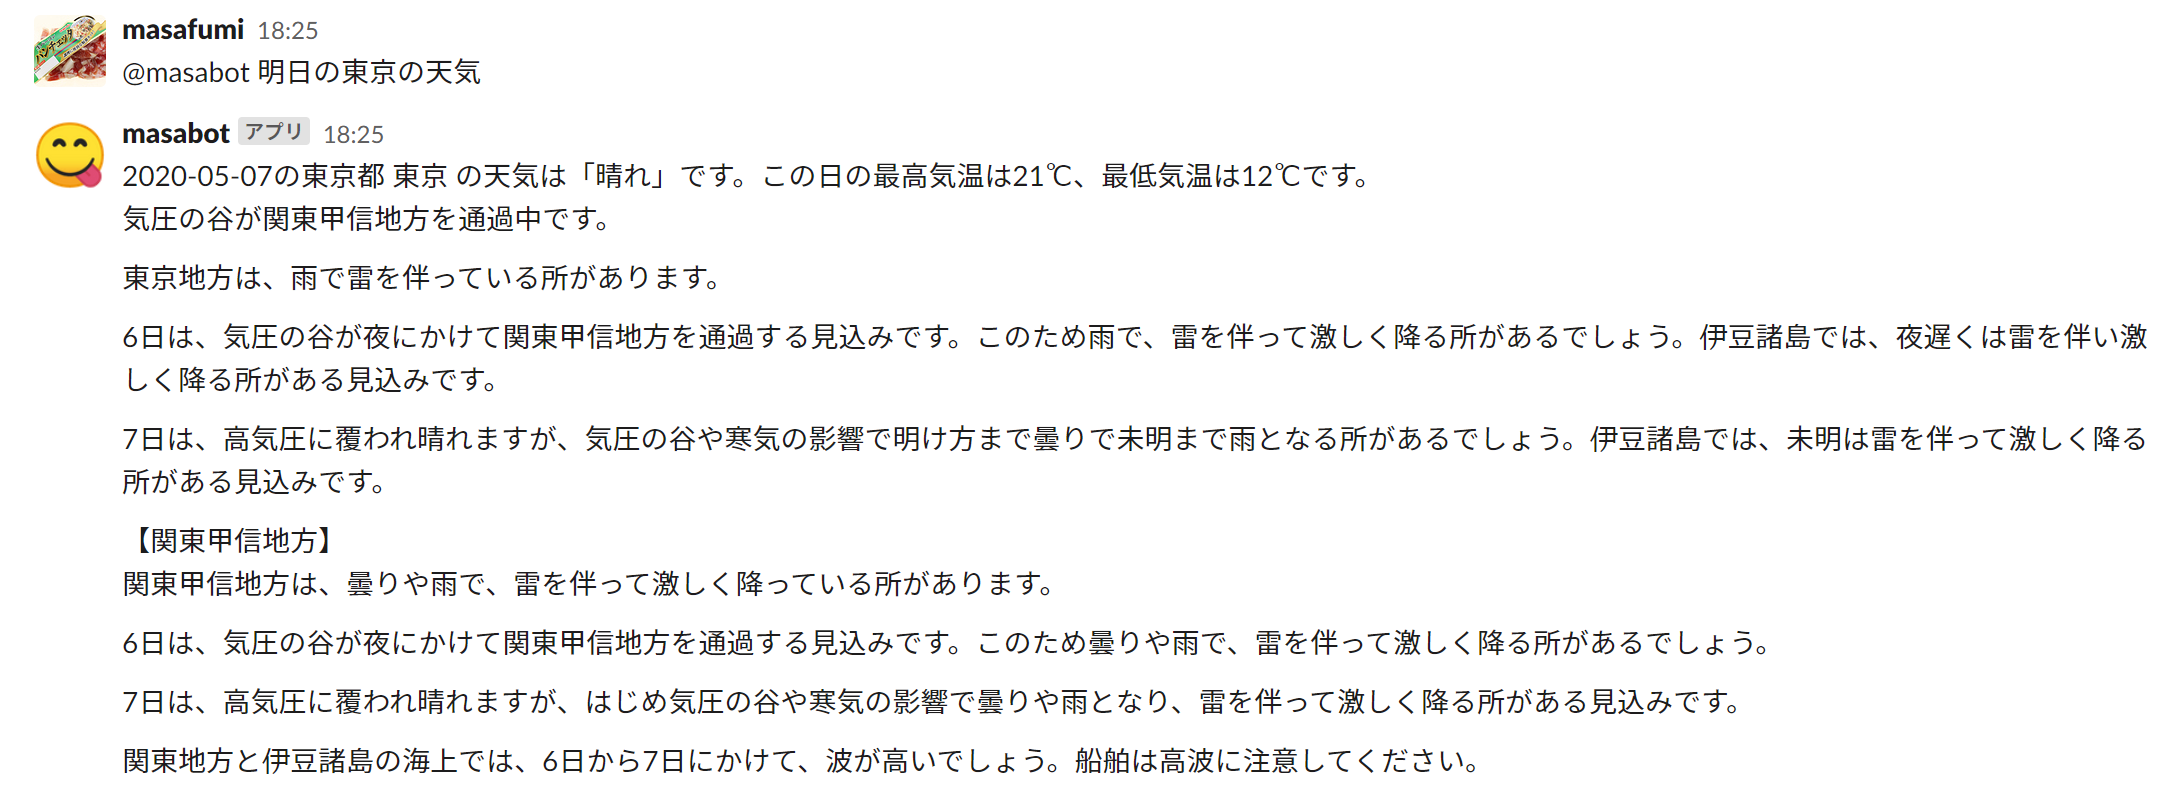
\includegraphics[width=1\textwidth]{figs/weather.png}
    \caption{ユーザが ``@masabot 明日の東京の天気''と投稿したときのSlackBotの返信}
    \label{fig:weather}
\end{figure}
この機能を使用するにあたって,ユーザが指定できる ``(日にち)''には, ``今日'', ``明日'', ``明後日''の3種類のうちのいずれかを入力する.
 ``(都道府県名)''には, ``東京''や ``岡山''など,日本の都道府県名を1つ入力する.
また, ``北海道''は ``道''という文字を含めて ``(都道府県名)''に入力する.
\end{description}
ユーザが(機能1),(機能2)を使用するために必要な文字列以外の文章を,Slackに投稿したとき,本プログラムは以下の文章を返信する.
\begin{verbatim}
   こんにちは、masabotです。        
   "@masabot 「○○○」と言って"と投稿した場合、"○○○"と返信します。
   天気予報を知りたいときは、"@masabot □□の△△の天気" 
   (□□は「今日」「明日」「明後日」のいずれか)(△△は都道府県名) と投稿してください。
   この日の指定した都道府県の天気を返信します。
\end{verbatim}


\section{動作環境}\label{sec:environment}
本プログラムの動作環境を表\ref{tab:2}に示す.
\begin{table}[h]
  \begin{center}
    \caption{動作環境}\label{tab:2}
%    \ecaption{Operating environment.}
    \begin{tabular}{l|l}
      \hline\hline
      \multicolumn{1}{l|}{項目} & \multicolumn{1}{l}{内容}\\
      \hline
      OS & Ubuntu 18.04.2 LTS\\
      CPU & Intel(R) COre(TM) m3-6Y30 CPU @ 0.90GHz\\
      メモリ & 4.0GB\\
      Ruby & ruby 2.5.5p157\\
      Gem & activesupport 6.0.2.2\\
     & bundler 2.1.4\\
     & json 2.1.0\\
     & openssl 2.1.2\\
     & rack 2.2.2, 2.0.4\\
     & rack-protection 2.0.8.1, 2.0.1\\
     & sinatra 2.0.8.1, 2.0.1\\
     & tilt 2.0.10, 2.0.8\\
      \hline
    \end{tabular}
  \end{center}
\end{table}


\section{環境構築}
本プログラムを実装するための環境の構築手順を以下に記述する.
\begin{enumerate}
\item SlackのIncoming WebHookの設定
\item SlackのOutgoing WebHookの設定
\item Herokuアカウントの作成と設定
\end{enumerate}
上記の手順の詳細の構築方法を以下に記述する.

\subsection{SlackのIncoming WebHookの設定}\label{sec:Incoming}
SlackにおけるIncoming WebHookの設定を以下の手順で行う.
\begin{enumerate}
\item 自分のSlackアカウントにログインする.
\item Slackの左上のメニューを開き,「その他管理項目」の「アプリを管理する」を開く.
\item カスタムインテグレーションから,「Incoming WebHook」を開く.
\item 「Slackに追加」した後,Incoming WebHookがメーセージを投稿するチャンネルを選択し,インテグレーションを追加する.
\item\label{enum:Heroku_URL} 名前をカスタマイズする.
  また,Webhook URLを\ref{sec:setup_Heroku}節(\ref{enum:in_URL})で使用するので控えておく.
\item 「設定を保存する」を選択する.
\end{enumerate}

\subsection{SlackのOutgoing WebHookの設定}
SlackにおけるOutgoing WebHookの設定を以下の手順で行う.
\begin{enumerate}
\item 自分のSlackアカウントにログインする.
\item Slackの左上のメニューを開き,「その他管理項目」から「アプリを管理する」を開く.
\item カスタムインテグレーションから,「Outgoing WebHook」を開く.
\item 「インテグレーションを追加する」を選択する.
\item Outgoing WebHookに関して,以下の設定を行う.
  \begin{enumerate}
  \item 「チャンネル」にて,ユーザが投稿した特定の文字列を監視するチャンネルを設定する.
  \item 「引き金となる言葉」にて,WebHookが動作する契機となる文字列を入力する.
  \item 「名前をカスタマイズ」にて,設定するOutgoing WebHookの名前を入力する.
  \end{enumerate}
\item 「設定を保存する」を選択する.
\end{enumerate}

\subsection{Herokuアカウントの作成と設定}\label{sec:setup_Heroku}
Herokuアカウントの作成と設定を以下の手順で行う.
\begin{enumerate}
\item 以下のURLよりHerokuにアクセスし,「新規登録」よりHerokuアカウントを登録する.\\
  https://jp.heroku.com/
\item 登録したアカウントでログインし,「Getting Started on Heroku」にて,「Ruby」を選択する.
\item 以下のコマンドを実行し,Heroku CLIをインストールする.\\
 \verb|$ sudo snap install heroku --classic|
\item herokuコマンドを使用するために,以下のコマンドを実行し,パスを通す.\\
  \verb|$ export PATH=$PATH:/snap/bin/|
\item 以下のコマンドを実行し,Heroku CLIがインストールできていることを確認する.\\
  \verb|$ heroku version|
\item 以下のコマンドを実行し,Heroku CLIにログインする.\\
  \verb|$ heroku login|
\item\label{enum:app} 作成したアプリケーションのディレクトリに移動して,以下のコマンドを実行し,Heroku上にアプリケーションを生成する.\\
  \verb|heroku <create <myapp_name>|
  
  なお,アプリケーション名は小文字と数字,およびハイフンのみ使用できる.
\item 以下のコマンドで,生成したHerokuのアプリケーションが,登録されていることを確認する.\\
  \begin{verbatim}
    $ git remote -v
    heroku	https://git.heroku.com/<myapp_name>.git (fetch)
    heroku	https://git.heroku.com/<myapp_name>.git (push)
  \end{verbatim}
\item\label{enum:in_URL} 以下のコマンドを実行し,\ref{sec:Incoming}節(\ref{enum:Heroku_URL})で控えておいたIncoming WebHook URLを,Herokuの環境変数に追加する.\\
  \verb|$ heroku config:set INCOMING_WEBHOOK_URL="https://XXXXXXXXXXXX"|
\end{enumerate}

\section{使用方法}
本プログラムを使用するには,以下の手順で行う.
\begin{enumerate}
\item 以下に示すGitリポジトリから本プログラムを取得する.\\
  \verb|git@github.com/masafumi0612/BootCamp.git|

\item 以下のコマンドを用いて,本プログラムをHerokuにデプロイする.\\
  \verb|git push heroku master|
\end{enumerate}

\section{エラー処理}
(機能2)を使用する際に,投稿する文字列の中に(日にち)が含まれていないときや,使用できる ``今日'',``明日'',``明後日''以外の文字列を使用したとき, ``今日''の指定した都道府県の天気予報を返信する.
例えば, ``東京の天気''や``明々後日の東京の天気''という文字列を投稿した際は,今日の東京の天気予報を返信する.
また,投稿する文字列の中に都道府県名が含まれていないとき,本プログラムはの以下にように返信する.
\begin{verbatim}
   都道府県名を入力してください。
   天気予報を知りたいときは、"@masabot □□の△△の天気" 
   (□□は「今日」「明日」「明後日」のいずれか)(△△は都道府県名) と投稿してください。
   指定した日にちの都道府県の天気を返信します。
\end{verbatim}
これに当てはまる例として,ユーザが ``@masabot 明日の天気''という文字列を投稿したときが挙げられる.

\section{保証しない動作}
本プログラムの保証しない動作を以下に記述する. 
\begin{enumerate}
\item \ref{sec:environment}章に示した動作環境以外の環境で,本プログラムを実行したときの動作
\item 本プログラムが,SlackのOutgoing WebHook以外からPOSTリクエストを受け取って実行した際の動作
  
\end{enumerate}

\bibliographystyle{ipsjunsrt}
\bibliography{mybibdata}

\end{document}
